\section{Results}
\label{sec:results}

\subsection{Exact Static Tie}
\label{sec:exact_match}

Phi-3.5-Vision and LLaVA-OneVision-7B have identical measured static Attribute
accuracy,
\begin{equation}
\widehat A_{S,\mathrm{Attr}}(\mathrm{Phi})=
\widehat A_{S,\mathrm{Attr}}(\mathrm{LLaVA})=80.5\%,
\label{eq:exact_static_tie}
\end{equation}
but RA values of $84.95\%$ and $100.00\%$. Their absolute RA gap is therefore
$15.05$ pp (paired-bootstrap 95\% CI: $10.21$--$20.43$ pp), while their II
values differ by $10.75$ pp. This is a finite-evaluation separation, not a
claim of equal population accuracies.

\subsection{All One-Point Matched Pairs}
\label{sec:near_match}

The primary rule yields seven comparisons. Table~\ref{tab:main-matched-pairs}
reports the full census rather than a selected subset. Their descriptive median
absolute RA gap is $15.05$ pp; four gaps are at least $10$ pp, three exceed
$20$ pp, and one exceeds $30$ pp. The median II gap is only $1.01$ pp.
Qualifying pairs can share a judge and are not treated as independent
observations for inferential testing.

\begin{table*}[t]
\centering
\small
\caption{Complete primary $|\Delta A_S|\leq1$ pp within-factor matched-pair
census. Gaps are absolute percentage points.}
\label{tab:main-matched-pairs}
\begin{tabular}{llrrr}
\toprule
Factor & Pair & $\Delta A_S$ & $\Delta\mathrm{RA}$ & $\Delta\mathrm{II}$\\
\midrule
Count & Molmo--Phi & 1.00 & 1.37 & 1.91\\
Attribute & Phi--LLaVA & .00 & 15.05 & 10.75\\
Presence & Molmo--Idefics3 & .50 & 25.63 & .51\\
Presence & Molmo--InternVL & .50 & 25.63 & 1.01\\
Presence & Qwen--LLaVA & 1.00 & 2.00 & .00\\
Presence & Idefics3--InternVL & 1.00 & .00 & .50\\
Spatial & Skywork--Phi & .35 & 38.60 & 1.56\\
\bottomrule
\end{tabular}
\end{table*}

The census also shows that the result is neither a claim that every
accuracy-matched pair has a large RA gap nor a selection of only favorable
examples. The Count comparison has a $1.37$ pp RA gap, and the
Idefics3--InternVL Presence comparison has no observed RA gap. In contrast,
the Attribute tie and the two Molmo Presence comparisons yield gaps from
$15.05$ to $25.63$ pp, while the Spatial Skywork--Phi comparison reaches
$38.60$ pp. Static-score matching can therefore conceal large behavioral
differences, but it does not guarantee them.

The largest gap is Spatial Skywork--Phi: $38.60$ pp despite a $0.35$ pp static
difference. Because Spatial relevant edits have larger average pixel change
than their controls, we treat this as supportive rather than the headline case.
The exact Attribute tie is not explained by larger relevant edits: its average
relevant pixel-change fraction is $0.118$, versus $0.179$ for irrelevant edits.

\subsection{Behavioral Profiles and Prediction Transitions}
\label{sec:behavioral_profiles}
\label{sec:prediction_transitions}
\FloatBarrier

\begin{figure*}[t]
\centering
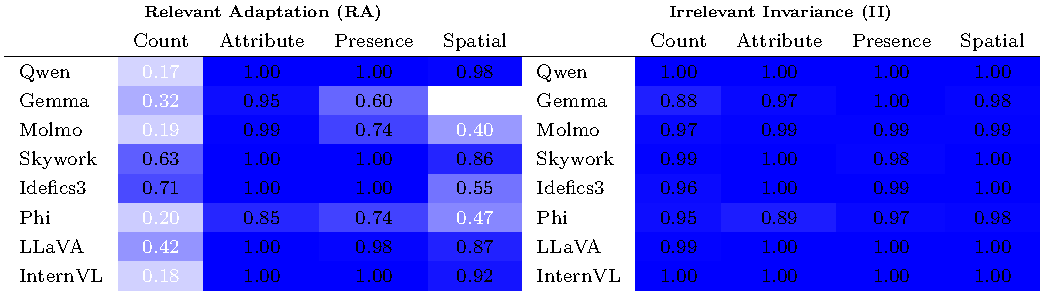
\includegraphics[width=.76\textwidth]{figures/dependency_fingerprint.pdf}
\caption{All $8\times4=32$ model--factor measurements. Relevant Adaptation
(RA) varies widely; Irrelevant Invariance (II) is predominantly high. Both are
conditional on a correct audit-base decision.}
\label{fig:behavioral_landscape}
\end{figure*}

Across all 32 cells, RA ranges from $0$ to $1$, whereas II ranges from about
$0.876$ to $1$ (Fig.~\ref{fig:behavioral_landscape}). High invariance therefore
does not imply appropriate adaptation. Qwen illustrates the distinction: it has
RA/II $=1/1$ on Attribute but RA/II $=.17/1$ on Count. It is correct on every
Count base image and follows the new preference on only $34/200$ relevant
edits. In the remaining $166/200$ cases, it retains its base prediction even
though the gold label changes, exactly the failure in
Eq.~\ref{eq:ra_retention}. Static accuracy is informative, but it does not
determine these selective response patterns.

\begin{figure*}[t]
\centering
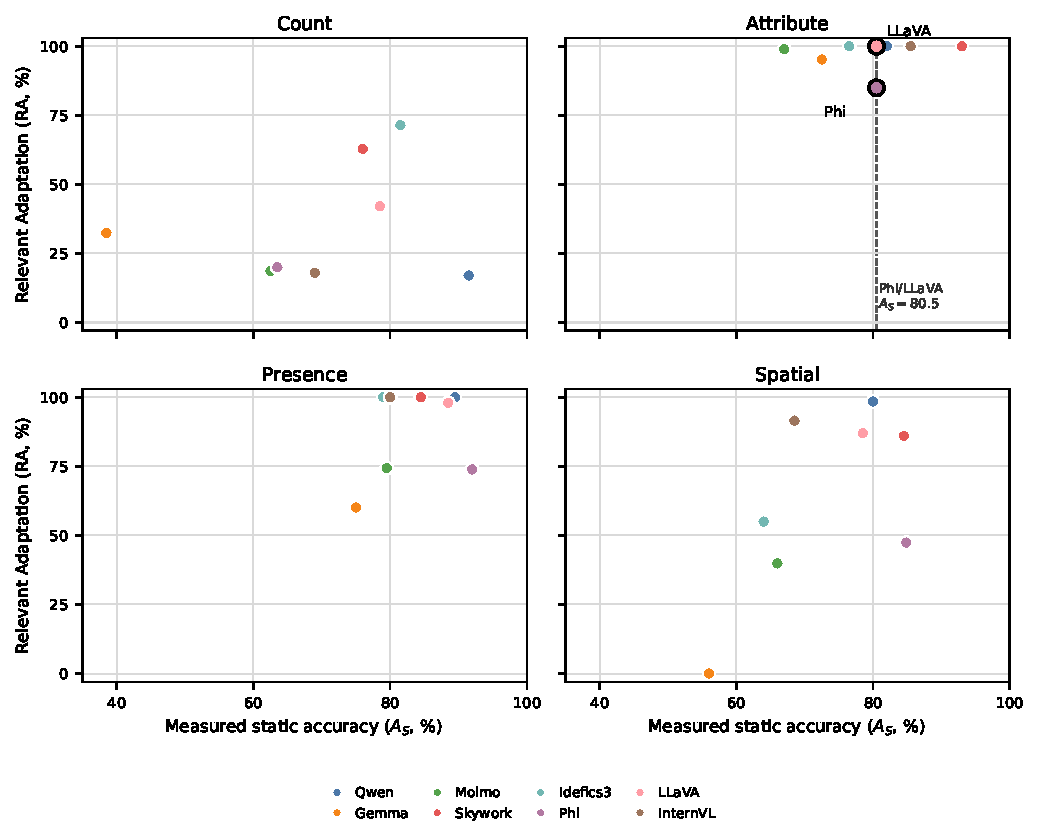
\includegraphics[width=.68\textwidth]{figures/static_vs_ra.pdf}
\caption{Measured static accuracy versus RA by factor. The Attribute panel
highlights the Phi--LLaVA exact tie at $80.5\%$ static accuracy and their
$84.95\%$ versus $100.00\%$ RA values.}
\label{fig:static_vs_ra}
\end{figure*}

\begin{figure*}[t]
\centering
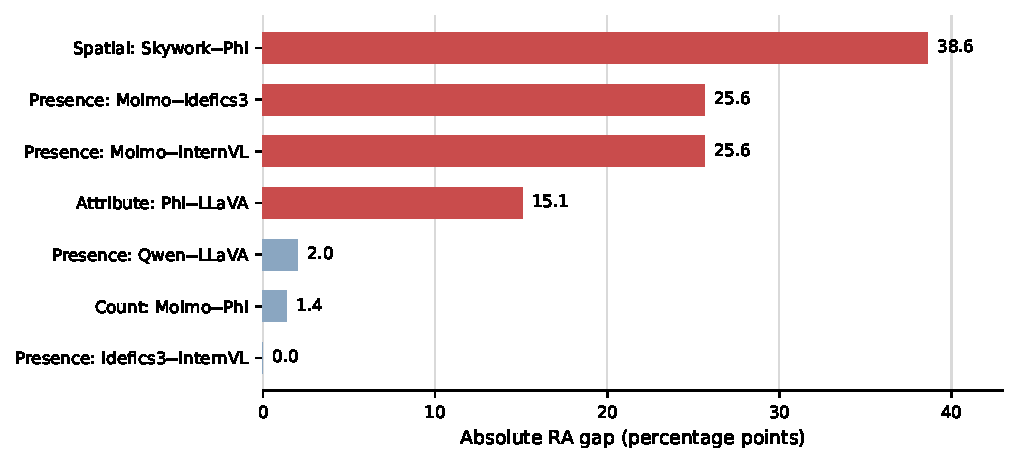
\includegraphics[width=.66\textwidth]{figures/matched_ra_gaps.pdf}
\caption{Ranked RA gaps for all seven primary matched pairs. Red bars mark
gaps of at least 10 pp.}
\label{fig:matched_pair_gaps}
\end{figure*}
